%===========================
% Chapitre 3 : Stratégies d'Arbitrage : Convexité, Portage et Limites de l'IA
%===========================
\chapter{Stratégies d'Arbitrage : Convexité, Portage et IA}
\label{chap:arb_convexite}
\textit{Enseigné par Julien Turc}

%--------------------------------------------------
\section{Genèse : L'arbitrage sur obligations convertibles}
%--------------------------------------------------

À l'origine de ce champ, un praticien remarque que les \textbf{obligations convertibles} (obligations d'entreprise échangeables en actions) étaient cotées sur le marché de la dette, sans que leur composante optionnelle (le droit de conversion en actions) ne soit correctement valorisée.

\begin{exemple}[Le premier arbitriste]
En utilisant le \textbf{modèle binomial de Rubinstein}, il identifie une sous-valorisation systématique. Sa stratégie :
\begin{enumerate}
    \item \textbf{Achat} d'obligations convertibles (sous-valorisées).
    \item \textbf{Vente à découvert} d'actions pour couvrir la composante « equity ».
\end{enumerate}
\textit{Contrainte opérationnelle :} à l'époque, il n'existait pas de marché de \textit{repo} organisé. Il fallait emprunter les actions directement auprès de gérants de portefeuille, avec des engagements jour par jour ou semaine par semaine.

\medskip
\textbf{Performance :} environ 80\% par an initialement, stabilisé autour de 30\% par an. Ce succès a ouvert la voie au champ de l'\textbf{arbitrage via obligations convertibles} (\textit{convertible bond arbitrage}).
\end{exemple}

Avec le temps, cette stratégie est devenue \textit{overcrowded} : trop de capitaux chassant les mêmes opportunités, le \textit{edge} a disparu. Les praticiens se sont alors tournés vers d'autres vecteurs d'arbitrage, notamment les \textbf{dérivés de crédit}.

%--------------------------------------------------
\section{La stratégie CDS-Actions}
%--------------------------------------------------

\subsection{Principe}

Lorsque le marché des CDS s'est développé, une nouvelle stratégie d'arbitrage a émergé, consistant à combiner :

\begin{itemize}
    \item \textbf{Achat de protection CDS} sur une entreprise (assurance contre le défaut).
    \item \textbf{Achat d'actions} de la même entreprise.
\end{itemize}

L'intuition est double :
\begin{itemize}
    \item Si l'entreprise \textbf{fait défaut} : le CDS est exercé et paie $(1-R) \times N$. La perte sur les actions est limitée (et peut être inférieure au gain CDS si le delta est bien calibré).
    \item Si l'entreprise \textbf{prospère} : la hausse des actions génère de l'alpha, et le coût du CDS reste limité (le spread reste faible).
\end{itemize}

Le résultat net est un profil de gain \textbf{convexe} : la position gagne dans les deux cas extrêmes, et ne perd modérément qu'en cas de stagnation.

\subsection{Le rôle du Chapter 11 américain}

\begin{remarque}
Aux États-Unis, une faillite d'entreprise se traduit par un dépôt en \textbf{Chapter 11} (restructuration judiciaire), qui n'entraîne \textbf{pas} nécessairement la disparition de l'action. L'entreprise continue souvent à coter pendant sa restructuration.

Conséquence pour la stratégie : même après déclenchement du CDS, l'action peut conserver voire retrouver de la valeur. Cela améliore le profil de gain net de la stratégie par rapport à une vision naïve.
\end{remarque}

%--------------------------------------------------
\section{La Convexité : le Graal de l'arbitriste}
%--------------------------------------------------

\subsection{Formalisation}

On note $S_0$ le prix initial de l'action. On construit une position :
\begin{itemize}
    \item Long $\delta$ actions (coût : $\delta S_0$).
    \item Acheteur de protection CDS (coût annuel : spread $s$, sur nominal $N$).
\end{itemize}

En simplifiant, le P\&L de la position est :
\[
\text{P\&L} = \underbrace{\delta \cdot (S_T - S_0)}_{\text{gain actions}} + \underbrace{\mathbb{1}_{\tau \le T} \cdot (1-R) \cdot N - s \cdot T \cdot N}_{\text{gain net CDS}}
\]

Si l'on suppose que le spread de crédit $s$ est une fonction décroissante du prix de l'action ($s = f(S)$, avec $f$ décroissante), alors :
\begin{itemize}
    \item Quand $S \downarrow$ fortement : $f(S)$ monte, le CDS se valorise fortement.
    \item Quand $S \uparrow$ : les actions montent, fournissant le gain equity.
\end{itemize}

La position globale a un profil \textbf{concave par le bas} : l'exposition aux pertes est bornée, tandis que les gains potentiels sont non linéaires. C'est ce que l'on appelle \textbf{capturer la convexité}.

\subsection{Représentation graphique de la convexité}

La figure~\ref{fig:convexite} représente le mark-to-market de la position combinée en fonction du prix de l'action $S$, centré sur $S_0$.

\begin{figure}[htbp]
    \centering
    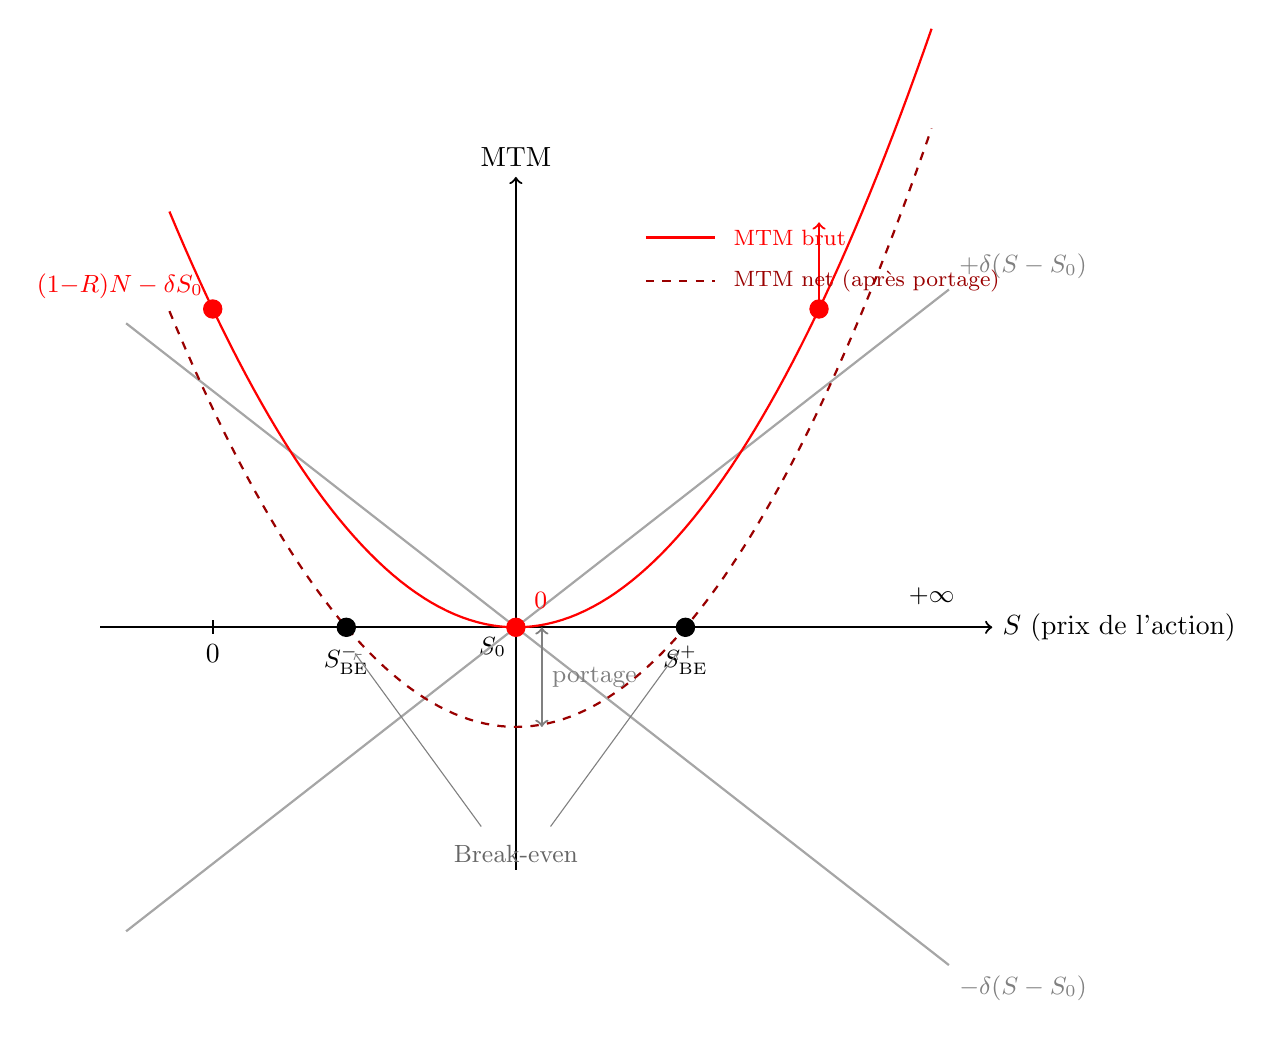
\begin{tikzpicture}[scale=1.1]
        % ===== AXES =====
        \draw[->, thick] (-4.8, 0) -- (5.5, 0) node[right] {$S$ (prix de l'action)};
        \draw[->, thick] (0, -2.8) -- (0, 5.2) node[above] {MTM};

        % --- Reference ticks on x-axis ---
        % S=0 (default): x = -3.5
        \draw[thick] (-3.5, 0.08) -- (-3.5, -0.08) node[below] {$0$};
        % S_0: origin
        \node[below left, font=\small] at (0, 0) {$S_0$};
        % infinity arrow on right
        \node[above, font=\small] at (4.8, 0.15) {$+\infty$};

        % ===== TWO LINEAR DELTA LINES (the "X") =====
        % Slope +delta (equity component): y = 0.78 * x
        \draw[thick, gray!70] (-4.5, -3.51) -- (5.0, 3.9)
            node[above right, font=\small, gray] {$+\delta(S - S_0)$};
        % Slope -delta (CDS component): y = -0.78 * x
        \draw[thick, gray!70] (-4.5, 3.51) -- (5.0, -3.9)
            node[below right, font=\small, gray] {$-\delta(S - S_0)$};

        % ===== RED CURVE : gross convex P&L (before carry) =====
        % f(x) = 0.30 * x^2  (parabola, min=0 at S_0)
        % Intersects delta lines when 0.30x^2 = 0.78|x| => |x| = 2.6
        \draw[thick, red]
            plot[domain=-4.0:4.8, samples=100] (\x, {0.30*\x*\x});

        % ===== DASHED CURVE : net P&L after carry costs =====
        % g(x) = 0.30 * x^2 - 1.15  (shifted down by carry C = 1.15)
        \draw[thick, red!60!black, dashed]
            plot[domain=-4.0:4.8, samples=100] (\x, {0.30*\x*\x - 1.15});

        % ===== 3 KEY POINTS ON THE RED CURVE =====
        % Point 1 : S=0 (default scenario, x=-3.5)
        \filldraw[red] (-3.5, {0.30*3.5*3.5}) circle (3pt);
        \node[above left, red, font=\small] at (-3.5, {0.30*3.5*3.5})
            {$(1{-}R)N - \delta S_0$};

        % Point 2 : S = S0 (x=0), minimum of the curve
        \filldraw[red] (0, 0) circle (3pt);
        \node[above right, red, font=\small] at (0.1, 0.1) {$0$};

        % Point 3 : S large (x=3.5), symmetric
        \filldraw[red] (3.5, {0.30*3.5*3.5}) circle (3pt);
        % upward arrow suggesting +inf
        \draw[->, red, thick] (3.5, {0.30*3.5*3.5+0.1}) -- (3.5, {0.30*3.5*3.5+1.0});

        % ===== CARRY ANNOTATION (vertical gap between curves at x=0) =====
        \draw[<->, thick, black!50] (0.3, -1.15) -- (0.3, 0)
            node[right, midway, font=\small] {portage};

        % ===== BREAK-EVEN POINTS (g(x)=0 => x=±sqrt(1.15/0.30)=±1.958) =====
        \def\xBE{1.958}
        \filldraw[black] (-\xBE, 0) circle (3pt);
        \filldraw[black] ( \xBE, 0) circle (3pt);
        \node[below, font=\small] at (-\xBE, -0.1) {$S^-_{\mathrm{BE}}$};
        \node[below, font=\small] at ( \xBE, -0.1) {$S^+_{\mathrm{BE}}$};

        % Arrows from "Break-even" label to the two points
        \node[below, font=\small, black!60] at (0, -2.4) {Break-even};
        \draw[->, black!50, thin] (-0.4, -2.3) -- (-\xBE+0.1, -0.3);
        \draw[->, black!50, thin] ( 0.4, -2.3) -- ( \xBE-0.1, -0.3);

        % ===== LEGEND =====
        \draw[thick, red]            (1.5, 4.5) -- (2.3, 4.5);
        \draw[thick, red!60!black, dashed] (1.5, 4.0) -- (2.3, 4.0);
        \node[right, font=\footnotesize, red]           at (2.4, 4.5) {MTM brut};
        \node[right, font=\footnotesize, red!60!black]  at (2.4, 4.0) {MTM net (après portage)};

    \end{tikzpicture}
    \caption{Profil de convexité de la stratégie CDS-Actions. Les droites grises $\pm\delta(S-S_0)$ représentent les composantes linéaires (equity et CDS). La courbe rouge solide est le MTM brut (convexe). La courbe rouge pointillée est le MTM net après portage, créant deux points de break-even $S^-_{\mathrm{BE}}$ et $S^+_{\mathrm{BE}}$.}
    \label{fig:convexite}
\end{figure}

\textbf{Lecture du graphique :}
\begin{itemize}
    \item \textbf{Scénario de défaut} ($S \to 0$) : le CDS paie $(1-R)N$, l'action vaut 0. Le gain net est $(1-R)N - \delta S_0 > 0$ si $\delta$ est bien calibré.
    \item \textbf{Stagnation} ($S \approx S_0$) : pas de perte structurelle, mais le portage grignote la valeur.
    \item \textbf{Forte hausse} ($S \gg S_0$) : l'equity monte, le CDS coûte peu comparativement. Gain net croissant.
    \item \textbf{Break-evens} : deux niveaux de prix de l'action où le portage annule exactement le gain de convexité.
\end{itemize}

\subsection{Cas limite : la fraude Enron}

\begin{exemple}[Enron (2001)]
En cas de fraude massive, l'action disparaît brutalement ($S_T \to 0$) et le CDS est déclenché. Le CDS paie alors $(1-R) \times N$.

Lors du défaut Enron, le taux de recouvrement était de $R = 15\%$, soit $(1 - R) = 85\%$ du nominal.

Si la position comportait $\delta$ actions couvrant un CDS de nominal $N$, le gain net de la stratégie s'écrit :
\[
\text{Gain} = (1-R) \cdot N - \delta \cdot S_0 = 0.85 \cdot N - \delta \cdot S_0
\]
Tant que $\delta < \frac{(1-R) \cdot N}{S_0}$, la stratégie est gagnante. En pratique, si le delta était bien estimé (inférieur à $0.85$), le gain a été très significatif.
\end{exemple}

%--------------------------------------------------
\section{Portage et Roll-down : le coût du temps}
%--------------------------------------------------

\subsection{Le portage (\textit{Carry})}

Toute position en CDS a un \textbf{coût de portage} : la prime $s$ versée prorata temporis à chaque période. Si le défaut survient au bout de $t$ années, le coût total de portage est :
\[
\text{Coût de portage} = s \cdot t \cdot N
\]
Exemple : un CDS à $s = 45$ bps porté 6 mois coûte $45 \times 0.5 = 22.5$ bps de nominal. Ce n'est pas négligeable.

\subsection{Le Roll-down}

\begin{definition}[Roll-down]
Le \textbf{Roll-down} est le gain (ou la perte) en mark-to-market résultant du simple vieillissement d'un contrat le long d'une courbe de crédit inchangée. Il traduit le fait qu'à conditions de marché identiques, un contrat initialement de maturité $T$ devient de maturité $T - \Delta t$ après $\Delta t$ années.
\end{definition}

Si la courbe de spread est montante et concave (ce qui est le cas typique), le spread à $T - \Delta t$ ans est \textbf{inférieur} au spread à $T$ ans. Pour l'acheteur de protection initialement à $s_T$, son contrat vaut désormais $s_{T-\Delta t} < s_T$ sur le marché. Le gain en mark-to-market est :

\begin{tcolorbox}[colback=blue!5,colframe=blue!40,title=Formule du Roll-down]
\[
\text{Roll-down} \approx (s_T - s_{T-\Delta t}) \times \text{DV01}_{T - \Delta t}
\]
\end{tcolorbox}

\textit{Exemple numérique :} un CDS 5 ans acheté à 45 bps. Un an plus tard, la courbe n'a pas bougé ; le contrat est maintenant un 4 ans coté à 35 bps.
\[
\text{Roll-down} = (45 - 35) \times \text{DV01}_{4Y} = 10 \text{ bps} \times \text{DV01}_{4Y}
\]

\begin{figure}[htbp]
    \centering
    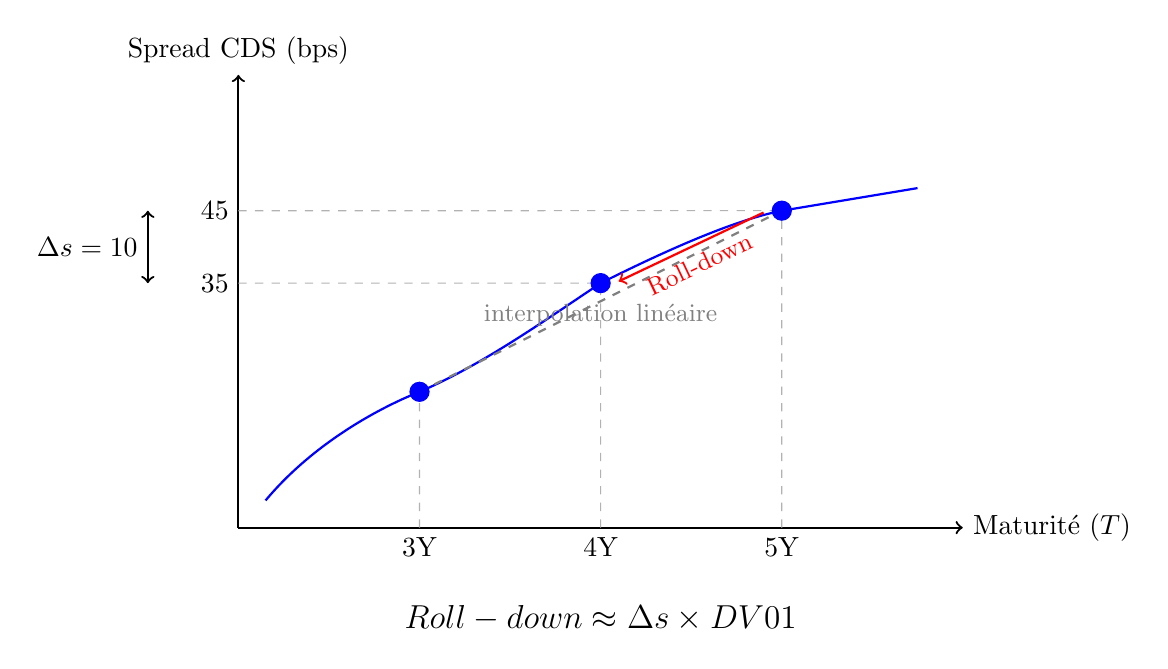
\begin{tikzpicture}[scale=1.15]
        % === Axes ===
        \draw[->, thick] (0,0) -- (8,0) node[right] {Maturité ($T$)};
        \draw[->, thick] (0,0) -- (0,5) node[above] {Spread CDS (bps)};

        % === Three key points (chosen to lie exactly on the curve) ===
        \coordinate (P3) at (2.0, 1.5);
        \coordinate (P4) at (4.0, 2.7);
        \coordinate (P5) at (6.0, 3.5);

        % === Concave CDS spread curve passing through the 3 points ===
        \draw[thick, blue]
            (0.3, 0.3)
            .. controls (0.8, 0.9) and (1.5, 1.3) .. (2.0, 1.5)
            .. controls (2.7, 1.8) and (3.4, 2.3) .. (4.0, 2.7)
            .. controls (4.8, 3.1) and (5.5, 3.4) .. (6.0, 3.5)
            .. controls (6.6, 3.6) and (7.2, 3.7) .. (7.5, 3.75);

        % === Chord from 3Y to 5Y (linear interpolation) ===
        \draw[dashed, gray, thick] (P3) -- (P5);
        \node[gray, font=\small] at (4.0, 2.35) {interpolation linéaire};

        % === Dashed vertical lines to x-axis ===
        \draw[dashed, gray!60] (2.0, 0) -- (P3);
        \draw[dashed, gray!60] (4.0, 0) -- (P4);
        \draw[dashed, gray!60] (6.0, 0) -- (P5);

        % === Dashed horizontal lines to y-axis (4Y and 5Y only) ===
        \draw[dashed, gray!60] (0, 2.7) -- (P4);
        \draw[dashed, gray!60] (0, 3.5) -- (P5);

        % === Dots on the curve ===
        \filldraw[blue] (P3) circle (3pt);
        \filldraw[blue] (P4) circle (3pt);
        \filldraw[blue] (P5) circle (3pt);

        % === X-axis labels ===
        \node[below] at (2.0, 0) {3Y};
        \node[below] at (4.0, 0) {4Y};
        \node[below] at (6.0, 0) {5Y};

        % === Y-axis labels ===
        \node[left] at (0, 2.7) {35};
        \node[left] at (0, 3.5) {45};

        % === DeltaS brace on y-axis ===
        \draw[<->, thick] (-1.0, 2.7) -- (-1.0, 3.5)
              node[midway, left] {$\Delta s = 10$};

        % === Roll-down arrow (5Y -> 4Y, along the curve) ===
        \draw[->, thick, red] (5.8, 3.48) -- (4.2, 2.72)
              node[midway, below, sloped, font=\small] {Roll-down};

        % === Formula below ===
        \node[align=center] at (4, -1.0)
              {\large $\text{Roll-down} \approx \Delta s \times \text{DV01}$};

    \end{tikzpicture}
    \caption{Roll-down sur la courbe de spread CDS. Le contrat 5Y (spread = 45 bps) devient un 4Y (spread = 35 bps) après 1 an à courbe inchangée. Le gain en mark-to-market vaut $\Delta s \times \text{DV01}_{4Y}$. La droite pointillée illustre l'interpolation linéaire entre 3Y et 5Y.}
    \label{fig:rolldown}
\end{figure}

\subsection{La DV01 : unité de risque en crédit}

\begin{definition}[DV01 — Dollar Value of a 01]
La \textbf{DV01} mesure la variation de la valeur mark-to-market d'un contrat de crédit pour un déplacement de \textbf{1 point de base} (0.01\%) du spread. Pour un CDS de maturité $T$ et de nominal $N$ :
\[
\text{DV01} = \frac{\partial V_{\text{CDS}}}{\partial s} \times 0.01\% = N \times \text{Risky Duration}(T) \times 0.01\%
\]
\end{definition}

\begin{remarque}
Contrairement aux produits de taux purs, la DV01 d'un CDS \textbf{incorpore le risque de crédit} dans son calcul. La Risky Duration est pondérée par la probabilité de survie :
\[
\text{Risky Duration}(T) = \int_0^T e^{-(r+\lambda)u} \, du
\]
Ce calcul nécessite d'injecter les probabilités de défaut ($\lambda$) et de survie ($e^{-\lambda t}$) dans la valorisation, ce qui le distingue d'une duration classique.
\end{remarque}

%--------------------------------------------------
\section{Les limites de l'IA face à la \textit{Small Data}}
%--------------------------------------------------

\subsection{Le problème de la non-stationnarité}

En finance, les données ne sont pas \textbf{stationnaires} : les relations entre variables (spreads, prix d'actions, taux) changent de régime au cours du temps (crises, changements réglementaires, cycles de taux). Contrairement aux lois de la physique, les lois de la finance \textit{varient}.

Cela pose un problème fondamental pour les modèles d'apprentissage automatique : un modèle calibré sur les données historiques d'un régime peut être totalement inadapté au régime suivant.

\subsection{Le mythe du Big Data en crédit}

\begin{remarque}
Un ordre de grandeur à retenir : un dataset multi-entreprises en crédit compte typiquement \textbf{20 ans de données quotidiennes} sur \textbf{150 entreprises}.
\[
20 \times 252 \times 150 = 756\,000 \text{ observations}
\]
C'est très loin des milliards de points nécessaires pour les réseaux de neurones profonds. Dans ce contexte, les méthodes \textbf{économes en données} (modèles structurels, formes réduites, ML classique, approches bayésiennes) sont souvent plus robustes que le Deep Learning.
\end{remarque}

Le tableau suivant résume la praticabilité des approches selon le contexte :

\begin{center}
\renewcommand{\arraystretch}{1.3}
\begin{tabular}{|l|c|c|}
\hline
\textbf{Approche} & \textbf{Adapté au crédit} & \textbf{Remarque} \\
\hline
Modèles structurels (Merton) & \checkmark & Peu de paramètres \\
\hline
ML classique (Lasso, SVM) & \checkmark & Robustes en petite dimension \\
\hline
Réseaux de neurones profonds & $\times$ & Trop de paramètres pour le volume de données \\
\hline
\end{tabular}
\end{center}

%--------------------------------------------------
\section{Le Modèle de Merton Revisité : la Dette comme Option}
%--------------------------------------------------

\subsection{Structure de bilan et équilibre de marché}

Le point de départ du modèle de Merton est une identité comptable fondamentale :

\begin{tcolorbox}[colback=blue!5,colframe=blue!40,title=Identité du bilan]
\[
V_t = E_t + D_t
\]
où $V_t$ est la valeur de marché des \textbf{actifs} de l'entreprise, $E_t$ la valeur des \textbf{actions} (equity), et $D_t$ la valeur de la \textbf{dette}.
\end{tcolorbox}

Puisque les actions cotent sur un marché, $E_t$ est observable. Merton fait alors l'hypothèse que les trois grandeurs sont des actifs de marché, et considère $V_t$ comme la variable latente sous-jacente, supposée suivre un mouvement Brownien géométrique :
\[
dV_t = \mu V_t \, dt + \sigma_A V_t \, dW_t
\]

\subsection{Représentation optionnelle}

On suppose que l'entreprise a émis une unique obligation zéro-coupon de nominal $K$, arrivant à maturité $T$.

\begin{itemize}
    \item Si $V_T \geq K$ : l'entreprise rembourse intégralement. Les actionnaires reçoivent $V_T - K > 0$.
    \item Si $V_T < K$ : défaut. Les créanciers récupèrent $V_T$ (liquidation). Les actionnaires reçoivent $0$.
\end{itemize}

\begin{definition}[Décomposition de Merton]
Les flux des deux types de porteurs peuvent s'écrire comme des dérivés :
\begin{align}
\text{Actionnaire :} & \quad \max(V_T - K, 0) = \text{Call}(V, K, T) \\
\text{Créancier :}   & \quad \min(V_T, K) = K - \max(K - V_T, 0) = K e^{-rT} - \text{Put}(V, K, T)
\end{align}
La dette risquée est donc un \textbf{zéro-coupon sans risque minoré d'un Put vendu} sur les actifs.
\end{definition}

\begin{figure}[htbp]
    \centering

    % ---- TOP : Balance Sheet ----
    \begin{subfigure}{\textwidth}
        \centering
        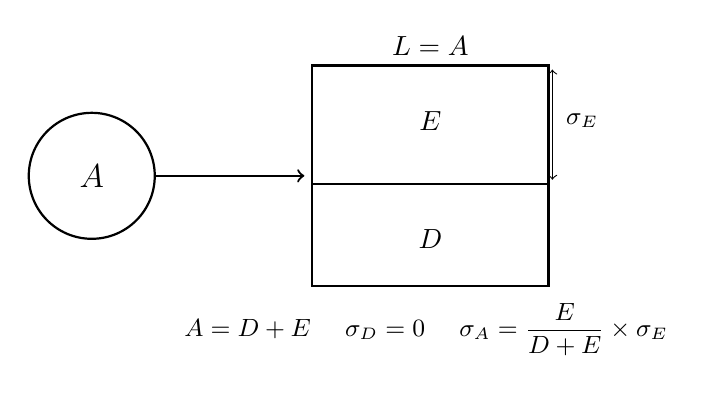
\begin{tikzpicture}[scale=1.0]
            % Asset circle
            \node[draw, circle, thick, minimum size=1.6cm, font=\large\bfseries]
                at (-2.8, 1.4) {$A$};
            \draw[->, thick] (-2.0, 1.4) -- (-0.1, 1.4);

            % Liabilities box
            \draw[thick] (0, 0) rectangle (3, 2.8);
            \draw[thick] (0, 1.3) -- (3, 1.3);
            \node[font=\bfseries] at (1.5, 2.1) {$E$};
            \node[font=\bfseries] at (1.5, 0.6) {$D$};

            % sigma_E brace
            \node[right, font=\small] at (3.1, 2.1) {$\sigma_E$};
            \draw[<->, thin] (3.05, 1.35) -- (3.05, 2.75);

            % L = A label
            \node[above, font=\bfseries] at (1.5, 2.8) {$L = A$};

            % Formulas below
            \node[below, align=left, font=\small] at (1.5, -0.1) {
                $A = D + E$ \quad
                $\sigma_D = 0$ \quad
                $\displaystyle\sigma_A = \frac{E}{D+E}\times\sigma_E$
            };
        \end{tikzpicture}
        \caption{Bilan de l'entreprise et relation entre volatilités}
    \end{subfigure}

    \vspace{1.5cm}

    % ---- BOTTOM : Debt Payoff Diagram ----
    \begin{subfigure}{\textwidth}
        \centering
        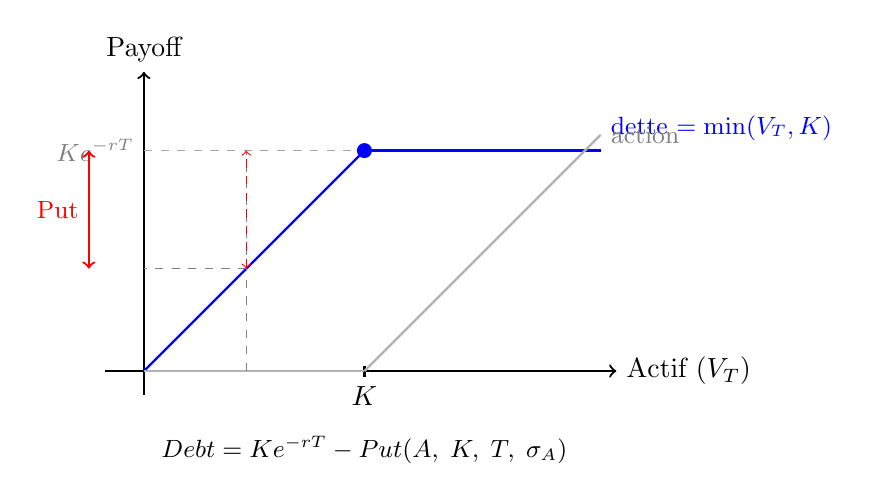
\begin{tikzpicture}[scale=1.0]
            % Axes
            \draw[->, thick] (-0.5, 0) -- (6.0, 0) node[right] {Actif ($V_T$)};
            \draw[->, thick] (0, -0.3) -- (0, 3.8) node[above] {Payoff};

            % Strike K
            \draw[thick] (2.8, 0.07) -- (2.8, -0.07) node[below] {$K$};

            % ZC level
            \draw[dashed, gray!70] (0, 2.8) -- (5.8, 2.8);
            \node[left, font=\small, gray] at (0, 2.8) {$K e^{-rT}$};

            % Debt payoff = min(V_T, K)
            \draw[thick, blue] (0, 0) -- (2.8, 2.8);
            \draw[thick, blue] (2.8, 2.8) -- (5.8, 2.8)
                node[above right, blue, font=\small] {dette $=\min(V_T, K)$};

            % Equity payoff (lighter)
            \draw[thick, gray!60] (0,0) -- (2.8, 0);
            \draw[thick, gray!60] (2.8, 0) -- (5.8, 3.0)
                node[right, gray, font=\small] {action};

            % Kink point
            \filldraw[blue] (2.8, 2.8) circle (2.5pt);

            % Dashed showing Put gap at V_T = 1.3
            \draw[dashed, gray] (1.3, 0) -- (1.3, 2.8);
            \draw[dashed, gray] (1.3, 1.3) -- (0,   1.3);

            % Put brace
            \draw[<->, thick, red] (-0.7, 1.3) -- (-0.7, 2.8)
                node[midway, left, red, font=\small] {Put};
            \draw[<->, thin, red, dashed] (1.3, 1.3) -- (1.3, 2.8);

            % Formula below
            \node[below, align=center, font=\small] at (2.8, -0.7)
                {$\text{Debt} = K e^{-rT} - \text{Put}(A,\; K,\; T,\; \sigma_A)$};
        \end{tikzpicture}
        \caption{Payoff de la dette à maturité $= \min(V_T, K)$ = zéro-coupon $-$ Put sur les actifs}
    \end{subfigure}

    \caption{Modèle de Merton : structure du bilan (haut) et représentation optionnelle de la dette (bas).}
    \label{fig:merton_bilan}
\end{figure}

\subsection{Déduction de la volatilité des actifs}

La volatilité des actifs $\sigma_A$ n'est pas directement observable. On la déduit via la relation entre l'équité et les actifs. Par Itô, la volatilité de l'équité $\sigma_E$ (observable via les options sur actions) est liée à $\sigma_A$ par :

\[
\sigma_E \cdot E_t = \frac{\partial E}{\partial V} \cdot \sigma_A \cdot V_t = \Delta_{\text{Call}} \cdot \sigma_A \cdot V_t
\]

Puisque la dette est supposée non volatile (dans l'approximation de Merton), on obtient :

\begin{tcolorbox}[colback=orange!5,colframe=orange!70,title=Volatilité des actifs (approximation)]
\[
\sigma_A \approx \frac{E_t}{V_t} \cdot \sigma_E = \frac{E_t}{E_t + D_t} \cdot \sigma_E
\]
Le ratio $E_t / (E_t + D_t)$ est l'inverse du \textbf{levier de marché} (\textit{market leverage}). Plus l'entreprise est endettée, plus $\sigma_A < \sigma_E$.
\end{tcolorbox}

\begin{remarque}
Cette hypothèse est circulaire : on price la dette en supposant que la dette a une volatilité nulle, alors que c'est précisément l'objet du pricing. En pratique, on résout le système d'équations non linéaires $\{E_t = \text{Call}(V_t, K, T, \sigma_A)\; ; \; \sigma_E E_t = \Delta \sigma_A V_t\}$ numériquement.
\end{remarque}

\subsubsection*{Instabilité numérique : la « vallée de colinéarité »}

L'observation que l'équité est un Call ($E_t = \text{Call}(V_t, K, T, \sigma_A)$) et que les options sur actions sont donc des \textbf{calls sur calls}, révèle une difficulté pratique fondamentale : les deux variables latentes $(V_t, \sigma_A)$ déterminent simultanément les actions \textit{et} la dette. Il existe une \textbf{vallée de colinéarité} dans l'espace des paramètres :

\begin{tcolorbox}[colback=red!5,colframe=red!50,title=Problème de colinéarité]
Il existe une famille de couples $(V_t, \sigma_A)$ qui laissent les observables $(E_t, \sigma_E)$ inchangés, tout en ayant un \textbf{impact très important sur le spread de crédit} modélisé. Cette dégénérescence rend l'optimiseur numériquement instable : de légères variations des inputs génèrent des spreads de crédit très différents.
\end{tcolorbox}

Concrètement, si l'on essaie d'ajuster à la fois le niveau et la volatilité des actifs pour coller à la fois aux actions et aux options sur actions, on obtient une multitude de solutions équivalentes pour les actions mais pas pour le crédit — rendant la calibration très sensible aux données initiales.

\subsection{Lien avec le spread de crédit et la convexité}

Dans ce cadre, \textbf{acheter de la protection CDS} revient à acheter un Put sur les actifs de l'entreprise. Le spread de crédit est structurellement fonction du prix de l'action (via $V_t = E_t + D_t$). Ce lien mécanique :
\begin{itemize}
    \item Justifie la stratégie CDS-Actions (cf. Section précédente).
    \item Garantit la \textbf{convexité positive} par construction du modèle.
\end{itemize}

%--------------------------------------------------
\section{La Courbe de Crédit et le Trade « Steepener »}
%--------------------------------------------------

\subsection{Problème d'extension : de la maturité unique à la courbe}

Le modèle de Merton standard pricing une seule maturité. En pratique, le marché du CDS génère une \textbf{courbe de spread} $s(T)$ pour $T \in \{1, 3, 5, 7, 10\}$ ans.

L'extension naïve — pricer un CDS $T$-ans avec une dette arrivant à maturité $T$ — crée des incohérences : les \textbf{taux forward de crédit peuvent devenir négatifs} pour certaines formes de courbe.

\subsection{La découverte du steepener (2003-2004)}

\begin{exemple}[Le trade Steepener]
Vers 2003, le marché CDS se développe principalement sur la maturité \textbf{5 ans}. Les courbes de crédit sont alors pratiquement \textbf{plates} : $s_{5Y} \approx s_{10Y}$.

Un Hedge Fund londonien demande aux banques des cotations sur le CDS \textbf{10 ans}. Les traders, faute de modèle de courbe, cotent le 10 ans au même niveau que le 5 ans.

\medskip
La stratégie d'arbitrage :
\begin{enumerate}
    \item \textbf{Achat de protection 10 ans} (spread $s_{10Y} \approx s_{5Y}$).
    \item \textbf{Vente de protection 5 ans} (spread $s_{5Y}$).
\end{enumerate}

\textbf{Portage net} $\approx 0$ (même spread payé et reçu).

\textbf{Rolldown sur le 5 ans} : voir section précédente — gain mécanique via la pente de la courbe lors du vieillissement du contrat.

\textbf{Rolldown sur le 10 ans} : nul car la courbe est plate (pas de pente exploitable).

\medskip
Résultat : stratégie à coût de portage nul, générant du rolldown sur la jambe 5 ans. \textbf{Arbitrage pur de portage.}
\end{exemple}

En agrégeant ces positions auprès de nombreuses banques, l'arbitriste a exercé une pression qui a progressivement « pentu » la courbe. Les Steepeners sont devenus un trade standard : jouer une augmentation de la pente $s_{10Y} - s_{5Y}$.

\begin{remarque}
Une fois la courbe pentue, le Steepener devient un trade de \textbf{convexité négative} (carry positif mais convexité courte), inverse du profil CDS-Actions.
\end{remarque}

\subsection{Construction DV01-neutre et P\&L du Steepener}

\subsubsection*{Hypothèse de déplacement parallèle}

En pratique, les traders ne travaillent pas à partir des taux forwards (qui représentent un scénario moyen dérivé de la courbe actuelle). Ils raisonnent en termes de \textbf{choc parallèle} : « que se passe-t-il si tous les spreads bougent de $+1\,\mathrm{bp}$ ? » C'est une hypothèse pragmatique qui correspond à la manière dont les systèmes de risque des hedge funds et banques étaient construits historiquement.

Sous cette hypothèse, si les deux spreads bougent de $+\Delta s$ :
\[
\text{P\&L}_{1\mathrm{bp}} = +\mathrm{DV01}(10) \cdot \Delta s \underbrace{- \mathrm{DV01}(5) \cdot \Delta s \cdot N_5 / N_{10}}_{\text{jambe 5Y}}
\]
Pour annuler ce risque directionnel (position \textbf{market-neutre sur les chocs parallèles}), on choisit le ratio de nominaux tel que les deux contributions se compensent.

Pour que le Steepener soit \textbf{neutre au risque de taux} (position non directionnelle sur le spread moyen), on construit la position de manière à ce que les deux jambes aient la même sensibilité en DV01.

\subsubsection*{Approximation du DV01}

Dans un cadre simplifié (taux sans risque $r$ et spread $s$ constants, coupons continus), le DV01 d'un CDS de maturité $T$ s'écrit :
\[
\mathrm{DV01}(T) = \int_0^T e^{-(r+s)t} \, dt = \frac{1 - e^{-(r+s)T}}{r+s}
\]

Pour des spreads et taux modérés ($r+s$ petit), on obtient l'approximation :\[
\mathrm{DV01}(T) \approx T \cdot e^{-sT}
\]
ce qui confirme que le ratio $\Delta \approx 10/5 = 2$ (la duration 10 ans est environ le double de la duration 5 ans) est une bonne approximation de premier ordre.

\begin{definition}[Ratio de couverture $\Delta$]
On note $N_5$ et $N_{10}$ les nominaux des jambes 5Y et 10Y. La condition de neutralité DV01 est :
\[
N_5 \times \mathrm{DV01}(5Y) = N_{10} \times \mathrm{DV01}(10Y)
\]
Le ratio de couverture est donc :
\begin{tcolorbox}[colback=blue!5,colframe=blue!40]
\[
\Delta = \frac{N_5}{N_{10}} = \frac{\mathrm{DV01}(10Y)}{\mathrm{DV01}(5Y)}
\]
\end{tcolorbox}
Comme $\mathrm{DV01}(10Y) > \mathrm{DV01}(5Y)$ (duration plus longue), on a $\Delta > 1$ : il faut vendre plus de nominal de 5Y que d'acheter de 10Y.
\end{definition}

\begin{figure}[htbp]
    \centering
    \begin{tikzpicture}[scale=1.1]
        % Axes
        \draw[->, thick] (0,0) -- (7.5,0) node[right] {Maturité};
        \draw[->, thick] (0,0) -- (0,4.5) node[above] {Spread CDS};

        % Spread curve (concave)
        \draw[thick, blue] (0.3,0.5)
            .. controls (1.5,1.5) and (2.5,2.5) .. (3.0,3.0)
            .. controls (3.8,3.5) and (5.5,3.8) .. (7.0,4.0);

        % 5Y point
        \coordinate (P5) at (3.0, 3.0);
        \filldraw[blue] (P5) circle (3pt);
        \draw[dashed, gray!60] (3.0, 0) -- (P5);
        \node[below] at (3.0, 0) {5Y};

        % 10Y point
        \coordinate (P10) at (6.0, 3.8);
        \filldraw[blue] (P10) circle (3pt);
        \draw[dashed, gray!60] (6.0, 0) -- (P10);
        \node[below] at (6.0, 0) {10Y};

        % DV01 arrows at each point (vertical, showing +1bp sensitivity)
        % At 5Y: shorter arrow (smaller DV01)
        \draw[->, thick, red!80] (3.0, 3.0) -- (3.0, 3.6)
            node[right, font=\small, red!80] {$+1\,\mathrm{bp} \Rightarrow \mathrm{DV01}(5)$};

        % At 10Y: taller arrow (larger DV01)
        \draw[->, thick, red!80] (6.0, 3.8) -- (6.0, 4.7)
            node[right, font=\small, red!80] {$+1\,\mathrm{bp} \Rightarrow \mathrm{DV01}(10)$};

        % Delta annotation between the two legs below x-axis
        \draw[<->, thick, black!70] (3.0, -0.5) -- (6.0, -0.5)
            node[midway, below, font=\small]
            {$\Delta = \dfrac{\mathrm{DV01}(10Y)}{\mathrm{DV01}(5Y)}$};
        \node[below left, font=\small] at (3.0, -0.45) {$-\mathrm{DV01}(5)$};
        \node[below right, font=\small] at (6.0, -0.45 ) {$+\mathrm{DV01}(10)$};

    \end{tikzpicture}
    \caption{Construction DV01-neutre du Steepener : vente de protection 5Y (nominal $\Delta \cdot N$) et achat de protection 10Y (nominal $N$), de façon à equaliser les sensibilités en DV01.}
    \label{fig:steepener_dv01}
\end{figure}

\subsubsection*{P\&L du Steepener}

Soit $M_5$ et $M_{10}$ les spreads de marché (en bps) des CDS 5Y et 10Y, et $\mathrm{RD}(T)$ le roll-down annuel sur la maturité $T$.

\begin{tcolorbox}[colback=orange!5,colframe=orange!60,title=P\&L du Steepener (DV01-neutre)]
\[
\text{Carry} = \Delta \times M_5 - M_{10}
\]
\[
\text{Roll-down} = \Delta \times \mathrm{RD}(5) - \mathrm{RD}(10)
\]
\end{tcolorbox}

\textit{Dans le cas initial (courbe plate, $M_5 = M_{10}$ et $\mathrm{RD}(10)=0$) :}
\[
\text{Carry} = (\Delta - 1) \times M_5 > 0 \quad \text{(puisque } \Delta > 1\text{)}
\]
\[
\text{Roll-down} = \Delta \times \mathrm{RD}(5) > 0
\]
Les deux composantes sont positives : c'est un arbitrage pur.

\subsubsection*{Comportements aux bornes : concavité du profil}

Le profil de P\&L du steepener en fonction de $M_5$ présente deux comportements extrêmes qui expliquent sa \textbf{concavité} :

\begin{center}
\renewcommand{\arraystretch}{1.3}
\begin{tabular}{|l|l|l|}
\hline
\textbf{Scénario} & \textbf{Condition} & \textbf{P\&L} \\
\hline
Défaut ($M_5 \to \infty$) & Entreprise en défaut & $-(\Delta - 1) \times \mathrm{LR}$ \\
\hline
Spreads nuls ($M_5 \to 0$) & Risque de crédit disparaît & $M_5 - M_{10} \leq 0$ (léger) \\
\hline
Zone intermédiaire & Carry + roll-down actifs & P\&L $\geq 0$ avec break-evens \\
\hline
\end{tabular}
\end{center}

\textbf{Interprétation :}
\begin{itemize}
    \item En cas de \textbf{défaut} ($M_5 \to \infty$) : on a vendu $(\Delta - 1)$ unités de plus de CDS 5Y que de CDS 10Y. La perte nette est $(\Delta - 1) \times \mathrm{LR}$ (taux de perte sur l'excédent non couvert).
    \item En cas de \textbf{spreads convergeant vers zéro} : le gain résiduel sur la jambe 5Y ($\Delta \cdot M_5 \cdot \mathrm{DV01}(5)$) et la perte sur le 10Y ($M_{10} \cdot \mathrm{DV01}(10)$) se compensent presque, laissant $M_5 - M_{10} \leq 0$.
    \item C'est l'ajout du \textbf{carry et du roll-down} (cf. tcolorbox P\&L) qui soulève le profil au-dessus de zéro dans la zone intermédiaire, créant deux break-evens sur les côtés.
\end{itemize}

\begin{figure}[htbp]
    \centering
    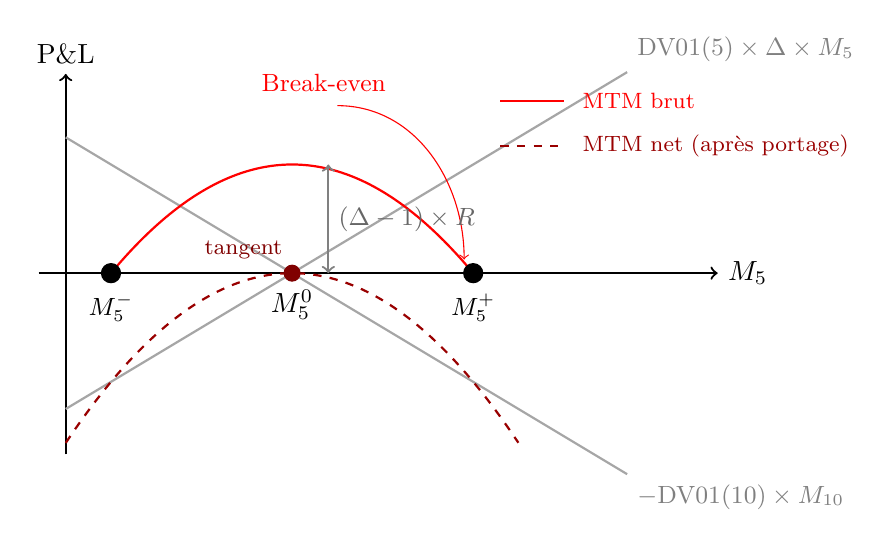
\begin{tikzpicture}[scale=1.15]

        % === Axes ===
        \draw[->, thick] (-0.3, 0) -- (7.2, 0) node[right] {$M_5$};
        \draw[->, thick] (0, -2.0) -- (0, 2.2) node[above] {P\&L};

        % Reference M5^0 at x=2.5
        \draw[thick] (2.5, 0.07) -- (2.5, -0.07) node[below] {$M_5^0$};

        % === X lines crossing at (2.5, 0) ===
        % Line 1: receive on 5Y leg — upsloping, slope +0.6
        \draw[thick, gray!70] (0, -1.5) -- (6.2, 2.22)
            node[above right, gray, font=\small] {$\mathrm{DV01}(5)\times\Delta\times M_5$};
        % Line 2: pay on 10Y leg — downsloping, slope -0.6
        \draw[thick, gray!70] (0, 1.5) -- (6.2, -2.22)
            node[below right, gray, font=\small] {$-\mathrm{DV01}(10)\times M_{10}$};

        % === GROSS dome (two break-evens): -0.3*(x-2.5)^2 + 1.2 ===
        % Zeros at x = 2.5 ± 2  →  x = 0.5 and x = 4.5
        \draw[thick, red]
            plot[domain=0.5:4.5, samples=100] (\x, {-0.3*(\x-2.5)*(\x-2.5) + 1.2});

        % === NET dome (tangent to x-axis at x=2.5): -0.3*(x-2.5)^2 ===
        \draw[thick, red!60!black, dashed]
            plot[domain=0.0:5.0, samples=100] (\x, {-0.3*(\x-2.5)*(\x-2.5)});

        % Tangent dot
        \filldraw[red!50!black] (2.5, 0) circle (2.5pt);
        \node[above left, red!50!black, font=\footnotesize] at (2.5, 0.05) {tangent};

        % === Break-even points (outer zeros of GROSS dome) ===
        \filldraw[black] (0.5, 0) circle (3pt);
        \filldraw[black] (4.5, 0) circle (3pt);
        \node[below, font=\small] at (0.5, -0.12) {$M_5^-$};
        \node[below, font=\small] at (4.5, -0.12) {$M_5^+$};

        % Break-even arrow and label
        \draw[->, thin, red] (3.0, 1.85) to[out=0,in=90] (4.4, 0.15);
        \node[above, red, font=\small] at (2.85, 1.9) {Break-even};

        % === Carry gap at M5^0 (vertical gap between two domes = carry cost) ===
        % At x=2.5: gross=1.2, net=0 → gap = 1.2
        \draw[<->, thick, black!50] (2.9, 0) -- (2.9, 1.2)
            node[right, midway, black!60, font=\small] {$(\Delta-1)\times R$};

        % === Legend ===
        \draw[thick, red]                  (4.8, 1.9) -- (5.5, 1.9);
        \draw[thick, red!60!black, dashed] (4.8, 1.4) -- (5.5, 1.4);
        \node[right, red, font=\footnotesize]           at (5.6, 1.9) {MTM brut};
        \node[right, red!60!black, font=\footnotesize]  at (5.6, 1.4) {MTM net (après portage)};

    \end{tikzpicture}
    \caption{Profil de P\&L du Steepener DV01-neutre. Les droites grises forment le «~X~». La courbe rouge pleine (brute) est un dôme avec deux break-evens $M_5^-$ et $M_5^+$ sur les côtés. La courbe rouge pointillée (nette, après portage) est décalée vers le bas et tangente à l'axe en $M_5^0$.}
    \label{fig:steepener_pl}
\end{figure}

%--------------------------------------------------
\section{Modélisation de la Courbe de Crédit : Deux Philosophies}
%--------------------------------------------------

La nécessité de modéliser une courbe entière (et non plus une maturité unique) a engendré un débat intellectuel analogue à celui des modèles de taux d'intérêt.

\subsection{Le point de vue « à l'ancienne » : le taux court (Vasicek)}

\begin{definition}[Modèle de Vasicek (1977)]
On modélise directement le \textbf{taux court} $r_t$ (ou l'intensité de défaut $\lambda_t$) par un processus à retour à la moyenne :
\[
dr_t = \kappa(\theta - r_t) \, dt + \sigma \, dW_t
\]
où $\kappa$ est la vitesse de retour à la moyenne $\theta$, et $\sigma$ la volatilité.
\end{definition}

L'avantage de cette approche est \textbf{interprétatif} : chaque paramètre a un sens économique.
\begin{itemize}
    \item $\theta$ : niveau long terme du taux (ou du spread).
    \item $\kappa$ : vitesse d'ajustement (mean-reversion).
    \item $\sigma$ : volatilité, qui génère une prime de risque et « bombe » la courbe.
\end{itemize}

La courbe $T \mapsto s(T)$ est entièrement déterminée par ces trois paramètres. C'est la même logique qui s'applique à Vasicek, Ho-Lee, Hull-White dans les taux.

\subsection{Le point de vue moderne : l'objet courbe (HJM)}

\begin{definition}[Cadre Heath-Jarrow-Morton (1992)]
Au lieu de modéliser un taux court, on modélise directement la \textbf{courbe entière} en faisant diffuser les taux forward instantanés $f(t, T)$ :
\[
df(t, T) = \mu(t, T) \, dt + \sigma(t, T) \, dW_t
\]
La condition d'absence d'arbitrage impose une contrainte sur $\mu$ (condition HJM) :
\[
\mu(t, T) = \sigma(t, T) \int_t^T \sigma(t, u) \, du
\]
\end{definition}

\begin{center}
\renewcommand{\arraystretch}{1.3}
\begin{tabular}{|l|p{5cm}|p{5cm}|}
\hline
& \textbf{Vasicek / Hull-White} & \textbf{HJM} \\
\hline
\textbf{Variable modélisée} & Taux court $r_t$ & Courbe entière $f(t,T)$ \\
\hline
\textbf{Interprétabilité} & Forte (paramètres économiques) & Faible (perte du sens de la pente) \\
\hline
\textbf{Élégance mathématique} & Moyenne & Très forte (cohérence no-arb par construction) \\
\hline
\textbf{Défaut} & Génère des distributions gaussiennes (taux négatifs) & Perd l'explication de l'origine de la pente \\
\hline
\end{tabular}
\end{center}

\begin{remarque}
Le débat HJM vs. Vasicek se retrouve dans tous les marchés de taux et de crédit. L'approche HJM est mathématiquement cohérente, mais le modèle à taux court conserve un avantage pédagogique : il décompose la courbe en \textbf{anticipation} (tendance centrale $\theta$) et en \textbf{prime de risque} (convexité générée par $\sigma$). Cette décomposition intuitive est précieuse pour l'analyse économique.
\end{remarque}

%--------------------------------------------------
\section{Vers un Modèle Cohérent : le Seuil de Défaut (Barrière)}
%--------------------------------------------------

\subsection{Problème des forwards négatifs dans Merton naïf}

Dans l'extension naïve du modèle de Merton à plusieurs maturités, on price un CDS de maturité $T$ en supposant que l'entreprise rembourse une dette arrivant exactement à la date $T$. Cette hypothèse conduit à des \textbf{probabilités de survie non monotones} : si la courbe de crédit n'est pas exactement cohérente avec ce schéma, les probabilités de défaut conditionnelles (forwards) peuvent devenir \textbf{négatives}.

\subsection{Le modèle à barrière : première formulation cohérente}

La solution est de remplacer la date de maturité unique par un \textbf{seuil de diffusion continu} : l'entreprise fait défaut \textit{dès que} la valeur de ses actifs $A_t$ passe en dessous d'un seuil $D$ (la barrière).

\begin{definition}[Temps de premier passage et probabilité de survie]
Soit $A_t$ la valeur des actifs de l'entreprise, diffusant selon un MBG. Le défaut survient au temps d'arrêt :
\[
\tau = \inf\{t \geq 0 : A_t \leq D\}
\]
La probabilité de survie à l'horizon $T$ est :
\[
\mathbb{Q}(\tau > T) = \mathbb{Q}\!\left(\forall t \leq T,\; A_t > D\right)
\]
\end{definition}

Cette formulation fait appel aux \textbf{formules de symétrie} du mouvement brownien (temps de premier passage, loi de l'arc-sinus) et garantit que les probabilités de survie sont décroissantes en $T$.

\begin{figure}[htbp]
    \centering
    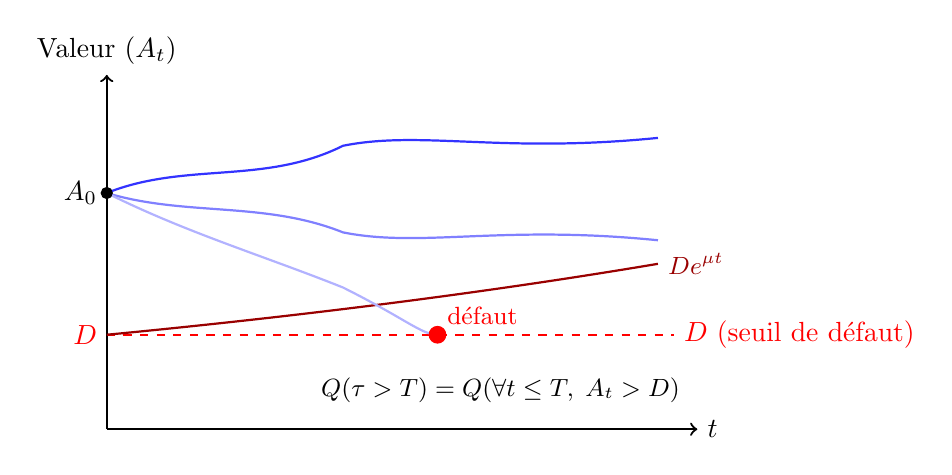
\begin{tikzpicture}[scale=1.0]
        % Axes
        \draw[->, thick] (0,0) -- (7.5,0) node[right] {$t$};
        \draw[->, thick] (0,0) -- (0,4.5) node[above] {Valeur ($A_t$)};

        % Barrier D
        \draw[dashed, red, thick] (0, 1.2) -- (7.2, 1.2)
            node[right, red] {$D$ (seuil de défaut)};
        \node[left, red] at (0, 1.2) {$D$};

        % Exponential debt De^(rt)
        \draw[thick, red!60!black]
            plot[domain=0:7, samples=60] (\x, {1.2*exp(0.08*\x)})
            node[right, font=\small, red!60!black] {$D e^{\mu t}$};

        % Several asset paths (Brownian diffusion from A0 > D)
        \draw[thick, blue!80]   (0,3.0) .. controls (1,3.4) and (2,3.1) .. (3,3.6)
                                        .. controls (4,3.8) and (5,3.5) .. (7,3.7);
        \draw[thick, blue!50]   (0,3.0) .. controls (1,2.7) and (2,2.9) .. (3,2.5)
                                        .. controls (4,2.3) and (5,2.6) .. (7,2.4);
        \draw[thick, blue!30]   (0,3.0) .. controls (1,2.5) and (2,2.2) .. (3,1.8)
                                        .. controls (3.8,1.4) and (4,1.2) .. (4.2,1.2);
        % Default event on last path
        \filldraw[red] (4.2, 1.2) circle (3pt);
        \node[above right, red, font=\small] at (4.2, 1.2) {défaut};

        % Initial value A0
        \filldraw[black] (0, 3.0) circle (2pt);
        \node[left] at (0, 3.0) {$A_0$};

        % Survival formula
        \node[align=left, font=\small] at (5.0, 0.5)
            {$\mathbb{Q}(\tau > T) = \mathbb{Q}(\forall t \le T,\; A_t > D)$};

    \end{tikzpicture}
    \caption{Modèle à barrière : $A_t$ diffuse à partir de $A_0 > D$. Le défaut survient au premier passage sous la barrière $D$ (fixe ou exponentielle $De^{\mu t}$). Les trois trajectoires illustrent des scénarios de survie (bleu) et de défaut (rouge).}
    \label{fig:barrier}
\end{figure}

\subsection{Avantage et limite du modèle à barrière}

\textbf{Avantage :} cohérence des probabilités de survie (monotones décroissantes), formules analytiques via la réflexion brownienne.

\textbf{Limite critique :} pour un mouvement brownien, la probabilité d'atteindre la barrière en temps infinitésimal est \textbf{nulle}. Cela implique :

\begin{tcolorbox}[colback=red!5,colframe=red!60,title=Problème du spread nul à court terme]
\[
\lim_{T \to 0} s(T) = 0 \quad \text{et} \quad \lim_{T \to 0} \frac{\partial s}{\partial T}(T) = 0
\]
Le spread de crédit et sa dérivée sont \textbf{tous deux nuls} à court terme. C'est une conséquence directe des propriétés du mouvement brownien : fondamentalement irréaliste pour les marchés.
\end{tcolorbox}

%--------------------------------------------------
\section{Formes de la Courbe de Crédit : Pathologies et Solutions}
%--------------------------------------------------

\subsection{Courbe en « chapeau de Napoléon » (dette constante)}

Si le seuil $D$ est \textbf{constant} et qu'on laisse la diffusion de $A_t$ agir sur le long terme, l'enveloppe parabolique des trajectoires devient de plus en plus large. La probabilité de survie à long terme \textit{diminue}, ce qui génère une courbe de spread en cloche (\og chapeau de Napoléon \fg) — non réaliste.

\begin{center}
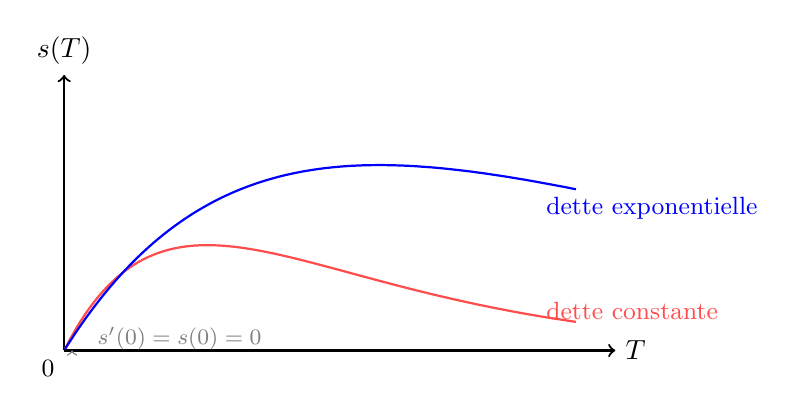
\begin{tikzpicture}[scale=1.0]
    \draw[->, thick] (0,0) -- (7,0) node[right] {$T$};
    \draw[->, thick] (0,0) -- (0,3.5) node[above] {$s(T)$};
    % Null slope near zero (tangent to x-axis)
    % Napoleon hat curve (rises then falls)
    \draw[thick, red!70] plot[domain=0.01:6.5, samples=100]
        (\x, {2.0 * \x * exp(-0.55*\x)});
    \node[right, red!70, font=\small] at (6.0, 0.5) {dette constante};
    % Corrected rising curve (exponential debt)
    \draw[thick, blue] plot[domain=0.01:6.5, samples=100]
        (\x, {1.6 * \x * exp(-0.25*\x)});
    \node[right, blue, font=\small] at (6.0, 1.8) {dette exponentielle};
    % Zero at origin annotation
    \node[below left, font=\small] at (0,0) {$0$};
    \draw[<->, thin, gray] (0.1, 0) -- (0.1, 0.001)
        node[right, gray, font=\footnotesize] at (0.3, 0.15) {$s'(0)=s(0)=0$};
\end{tikzpicture}
\end{center}

\textbf{Solution :} supposer que la barrière croît exponentiellement : $D(t) = D_0 e^{\mu t}$ (la dette est refinancée à un taux $\mu$). Cela supprime la descente à long terme et donne une courbe \textbf{monotone croissante} — plus réaliste.

\subsection{Ajout d'un saut : résoudre le spread nul à court terme}

Pour corriger le spread nul à l'origine, on ajoute un \textbf{processus de Poisson} d'intensité $\lambda_0$ à la diffusion :

\begin{tcolorbox}[colback=blue!5,colframe=blue!40,title=Spread court terme avec saut]
\[
s(T) \underset{T \to 0}{\longrightarrow} (1-R) \cdot \lambda_0 = M_0
\]
\end{tcolorbox}

Ce résultat (dû à \textbf{Darrell Duffie}) constitue la relation fondamentale entre spread, intensité et taux de perte :
\[
\boxed{M_0 = \mathrm{LR} \times \lambda}
\]
où $\mathrm{LR} = (1-R)$ est le taux de perte (\textit{Loss Rate}) et $\lambda$ est l'intensité instantanée de défaut.

\begin{figure}[htbp]
    \centering
    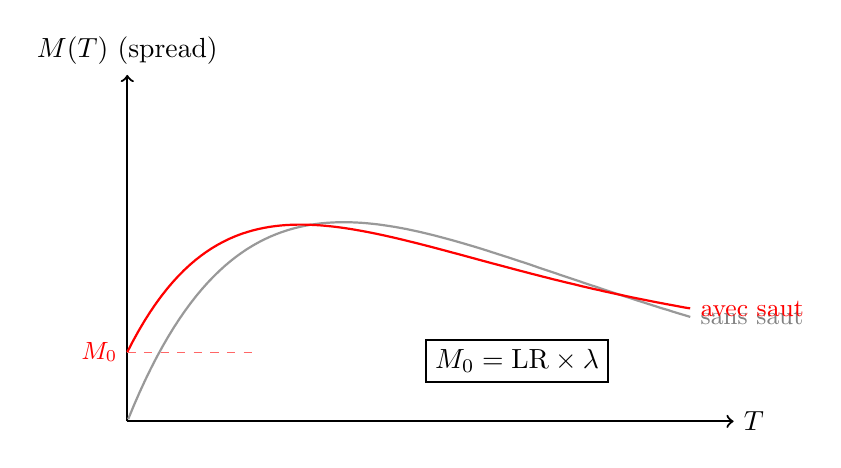
\begin{tikzpicture}[scale=1.1]
        % Axes
        \draw[->, thick] (0,0) -- (7.0,0) node[right] {$T$};
        \draw[->, thick] (0,0) -- (0,4.0) node[above] {$M(T)$ (spread)};

        % White curve: diffusion only (null at origin, null slope)
        \draw[thick, gray!80]
            plot[domain=0.01:6.5, samples=100]
                (\x, {2.5 * \x * exp(-0.40*\x)})
            node[right, gray, font=\small] {sans saut};

        % Red curve: diffusion + Poisson jump (non-null at origin)
        \draw[thick, red]
            plot[domain=0:6.5, samples=100]
                (\x, {0.8 + 2.0 * \x * exp(-0.50*\x)})
            node[right, red, font=\small] {avec saut};

        % M0 level annotation
        \draw[dashed, red!60] (0, 0.8) -- (1.5, 0.8);
        \node[left, red, font=\small] at (0, 0.8) {$M_0$};

        % Box with formula
        \node[draw, thick, fill=white, font=\normalsize] at (4.5, 0.7)
            {$M_0 = \mathrm{LR} \times \lambda$};

    \end{tikzpicture}
    \caption{Courbe de spread $M(T)$ en fonction de la maturité $T$. Sans saut (diffusion pure), $M(0)=0$ et $M'(0)=0$ : le spread converge vers zéro à l'origine. Avec un saut de Poisson d'intensité $\lambda_0$, le spread initial est non nul : $M_0 = \mathrm{LR} \times \lambda_0$.}
    \label{fig:spread_curve}
\end{figure}

\subsection{CreditGrades et processus de Lévy}

\begin{exemple}[CreditGrades (JP Morgan / Goldman Sachs, ~2002)]
Quants de banques d'investissement londoniennes ont proposé de rendre le seuil de dette $D$ \textbf{stochastique} : $D \sim \mathrm{LogNormal}$. Cette convolution introduit une incertitude sur la barrière et génère un spread non nul à l'origine.

Paramètres : $(A, D, T, \sigma_A)$ avec seuil log-normal. Le modèle a une \og jolie petite formule \fg{} fermée, mais ne résout pas le problème de la dérivée nulle.
\end{exemple}

\begin{exemple}[Processus Variance Gamma (Lévy)]
En remplaçant le mouvement brownien par un \textbf{processus Variance Gamma} $X_t = W_{\gamma(t)}$ (changement de temps aléatoire sur un brownien), on obtient un processus de Lévy avec sauts inférieurs, résolvant simultanément les deux problèmes ($s(0) \neq 0$ et $s'(0) \neq 0$).

Limitation pratique : dès qu'on sort du cas Variance Gamma, les distributions tempérées/semi-tempérées ne sont plus analytiquement traitables.
\end{exemple}

%--------------------------------------------------
\section{Le Modèle d'Intensité de Duffie : une Alternative Pragmatique}
%--------------------------------------------------

\subsection{L'idée fondamentale : paramétrer l'intensité directement}

Au lieu de modéliser la valeur des actifs $A_t$ (entité abstraite et non observable), on modélise directement \textbf{l'intensité de défaut} $\lambda_t$ comme une fonction du prix de l'action $S_t$ :

\begin{tcolorbox}[colback=blue!5,colframe=blue!40,title=Modèle d'intensité de Duffie]
\[
\lambda_t = f(S_t) = \left(\frac{L \cdot e^{\mu t}}{S_t}\right)^p + \lambda_0
\]
\end{tcolorbox}

L'interprétation est la suivante :
\begin{itemize}
    \item $\dfrac{L e^{\mu t}}{S_t} = \dfrac{\mathrm{Debt}(t)}{\mathrm{MarketCap}(t)}$ est le \textbf{levier de marché} (\textit{market leverage}), observable.
    \item $\mu$ : taux de croissance de la dette (\textit{debt growth rate}) — paramètre économique interprétable.
    \item $p$ : exposant de sensibilité, calibré sur les données de marché.
    \item $\lambda_0$ : intensité de fond (assure un spread non nul à court terme).
\end{itemize}

Ce modèle décompose la courbe de crédit en \textbf{scénario central} ($\mu$, le taux de croissance de la dette) et \textbf{prime de risque} ($p$, la sensibilité au levier).

\begin{remarque}
Pour les entreprises \textbf{investment grade} (levier faible, loin du seuil), le terme $(L/S)^p$ est très petit. L'intensité est dominée par $\lambda_0$, et le modèle se réduit à un modèle à intensité constante — équivalent à ignorer la structure de capital. Le message : pour l'investment grade, la \textbf{volatilité} (via l'impact sur $S_t$) est la variable clé, pas le levier.
\end{remarque}

%--------------------------------------------------
\section{Applications : Trades LBO et Structures de Courbe}
%--------------------------------------------------

\subsection{Le trade LBO (\textit{Leveraged Buy-Out})}

Un LBO est le rachat d'une entreprise par un fonds d'investissement qui finance l'acquisition principalement par dette, augmentant brutalement le levier de l'entreprise.

\begin{exemple}[Trade jackpot sur l'investment grade]
Une entreprise investment grade (faible levier, CDS bon marché) est identifiée comme candidate LBO. La position :
\begin{enumerate}
    \item \textbf{Achat de protection CDS} : si le LBO a lieu, le risque de crédit explose → le CDS se valorise fortement.
    \item \textbf{Achat d'actions} : le fonds d'investissement booste le prix de l'action en transférant le risque sur les créanciers.
\end{enumerate}
Résultat : gain simultané sur les deux jambes. La stratégie reproduit un profil convexe similaire à la figure~\ref{fig:convexite}.
\end{exemple}

\subsection{Inversion de courbe en cas de défaut imminent}

La courbe de spread $T \mapsto s(T)$ présente une structure caractéristique en fonction du niveau absolu de spread :

\begin{center}
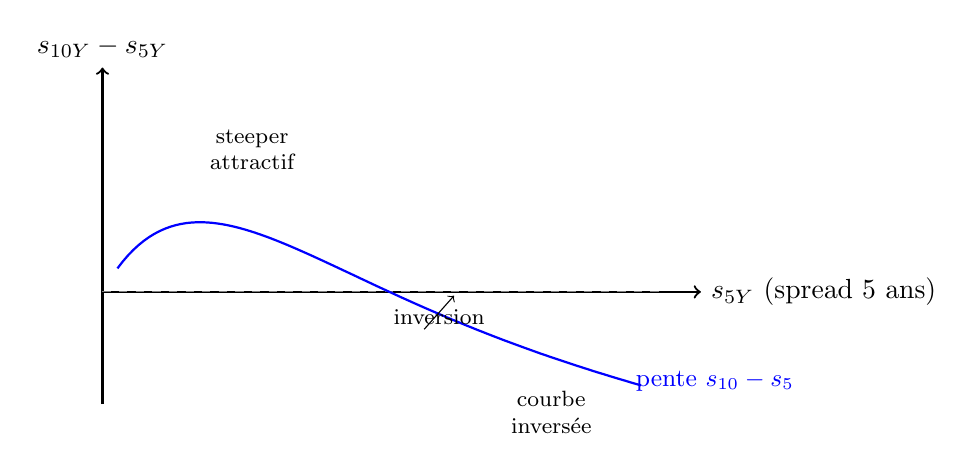
\begin{tikzpicture}[scale=0.95]
    \draw[->, thick] (0,0) -- (8.0,0) node[right] {$s_{5Y}$ (spread 5 ans)};
    \draw[->, thick] (0,-1.5) -- (0,3.0) node[above] {$s_{10Y} - s_{5Y}$};
    % Zero line
    \draw[dashed, gray] (0,0) -- (7.5,0);
    % Hump-shaped curve: starts at 0, rises, then falls negative
    \draw[thick, blue]
        plot[domain=0.2:7.2, samples=100]
            (\x, {2.0 * \x * exp(-0.6*\x) - 0.2*\x});
    \node[right, blue, font=\small] at (7.0, -1.2) {pente $s_{10}-s_5$};
    % Zero crossing annotation
    \node[below, font=\small] at (4.5, -0.1) {\footnotesize inversion};
    \draw[->, thin] (4.3, -0.5) -- (4.7, -0.05);
    % Region labels
    \node[above, font=\footnotesize, align=center] at (2.0, 1.5) {steeper\\attractif};
    \node[below, font=\footnotesize, align=center] at (6.0, -1.2) {courbe\\inversée};
\end{tikzpicture}
\end{center}

Quand $s_{5Y}$ est très élevé (probabilité de défaut élevée à court terme), la courbe \textbf{s'inverse} : $s_{5Y} > s_{10Y}$. La pente $s_{10Y} - s_{5Y}$ passe négative. Ce signal est la borne supérieure naturelle du trade Steepener.

%--------------------------------------------------
\section{Pricing par EDP dans le Modèle d'Intensité (Processus de Cox)}
%--------------------------------------------------

\subsection{Cadre général}

Dans un \textbf{processus de Cox} (processus de Poisson à intensité stochastique $\lambda_t$), le prix de l'action $S_t$ et l'indicateur de défaut $\mathbf{1}_{\tau \leq t}$ sont couplés. On définit les probabilités de survie conditionnelles :
\[
P(t, T) = \mathbb{E}\!\left[\exp\!\left(-\int_t^T \lambda_s \, ds\right) \Bigg| \mathcal{F}_t\right] \quad \text{(courbe de crédit)}
\]

\subsection{Pricing du CDS : décomposition en deux branches}

Le spread de marché $M$ d'un CDS satisfait l'équation de juste valeur :
\[
M \times \underbrace{\mathrm{DV01}}_{\text{branche premium}} = \underbrace{(1-R) \times \int_0^T (-dP(0,t))}_{\text{branche défaut}}
\]

\begin{definition}[DV01 dans un modèle d'intensité]
\[
\mathrm{DV01}(T) = \int_0^T P(0, t) \, dt
\]
où $P(0, t)$ est la probabilité de survie actualisée.
\end{definition}

\subsection{Pricing des options : EDP de Black-Scholes généralisée}

Dans ce cadre, le prix $V(t, S)$ d'une option sur action satisfait une EDP intégrant le risque de défaut :

\[
\frac{\partial V}{\partial t} + \frac{\sigma^2 S^2}{2} \frac{\partial^2 V}{\partial S^2} + (r - \lambda \cdot \mathrm{LR}) S \frac{\partial V}{\partial S} - (r + \lambda) V + \lambda \cdot V_{\mathrm{défaut}} = 0
\]

où $V_{\mathrm{défaut}}$ est la valeur résiduelle de l'option en cas de défaut (typiquement 0 pour un call, $K$ pour un put).

\begin{remarque}
La présence du terme $\lambda \cdot V_{\mathrm{défaut}}$ distingue fondamentalement ce pricing du Black-Scholes standard. Elle induit une \textbf{skew de crédit} sur les options : les puts profonds sont plus chers que prédit par Black-Scholes, en raison du risque de saut de l'action à zéro lors du défaut.
\end{remarque}
